\subsection*{Aufgabe 3 - Trajektorienplanung}


Die vorliegende Trajektorienplanung beschäftigt sich mit der Definition und Berechnung von Trajektorien für einen Robotermanipulator. Das Ziel der Trajektorie wird dabei in globalen Koordinaten angegeben und ist durch den Vektor \( y_{\text{end\_glob}} \) definiert. Dieser Vektor repräsentiert die gewünschte Endposition des Endeffektors des Roboters.

\begin{verbatim}
    Ziel in globalen Koordinaten
    y_end_glob = [4*sqrt(6)-4*sqrt(2)-10; ...
                 -4*sqrt(6)-4*sqrt(2)-10*sqrt(3); 0]/125;
\end{verbatim}

Um die Trajektorie zu planen, müssen zuerst die globalen Koordinaten in Gelenkwinkel umgerechnet werden. Aus der Kinematik ergibt sich folgende Funktion zum Bestimmen der Gelenkwinkel. Dabei ist \(q(1)\) der Winkel \(\alpha\) und \(q(2)\) der Winkel \(\beta\). Die Funktion \texttt{pos\_endeff} gibt die Endposition in globalen Koordinaten abhängig von den Gelenkwinkeln \(\alpha\) und \(\beta\) an.  Weiterhin berechnet die Funktion \texttt{to\_endeff} den Abstand zwischen der Endeffektorposition und der Startposition, abhängig von den Gelenkwinkeln. Sobald \texttt{to\_endeff} Null ist, befindet sich der Endeffektor an der gewünschten Position. Die Funktion \texttt{q\_end} löst dies mit den Anfangsbedingungen \(q_0\) und gibt die Gelenkwinkel für die Endposition zurück.

\begin{verbatim}
    pos_endeff = @(q) 4/25*[sin(q(1)) + 4/5*sin(q(1)+q(2)); ...
    - cos(q(1)) - 4/5*cos(q(1)+q(2)); 0];
    to_endeff = @(q) pos_endeff(q) - y_end_glob;
    q_0 = [y_0(1); y_0(3)];
    q_end = fsolve(to_endeff, q_0);
\end{verbatim}

Mit den berechneten Winkeln kann die Trajektorienplanung beginnen. Wir haben uns für einen quintic spline entschieden, da dort sowohl Lage, Geschwindigkeit und Beschleunigung der Start- und Endlage vorgegeben werden können.
 Es müssen die Koeffizienten der Polynome 5.ten Grades berechnet werden.

 \begin{verbatim}
    a_poly = @(t)  a_coef(1) + a_coef(2)*(t-t_0) + a_coef(3)*(t-t_0).^2 
                 + a_coef(4)*(t-t_0).^3 + a_coef(5)*(t-t_0).^4 + a_coef(6)*(t-t_0).^5;
   
    b_poly = @(t)  b_coef(1) + b_coef(2)*(t-t_0) + b_coef(3)*(t-t_0).^2
                 + b_coef(4)*(t-t_0).^3 + b_coef(5)*(t-t_0).^4 + b_coef(6)*(t-t_0).^5;
\end{verbatim}

Die Anfangs- und Endbedingungen werden in \texttt{a\_init} und \texttt{b\_init} definiert. Dabei sind die Lage, die Geschwindigkeit und die Beschleunigung für Anfangs- und Endlage beschrieben.

\begin{verbatim}
    t_0 = tspan(1);
    t_end = tspan(2);
    a_init = [ q_0(1); y_0(2); 0;  q_end(1); 0; 0];
    b_init = [ q_0(2); y_0(4); 0;  q_end(2); 0; 0];
\end{verbatim}


Die A-Matrix wird durch das Ableiten des Polynoms und Einsetzen des Startzeitpunktes und des Endzeitpunktes für t gebildet. 

\begin{equation*}
	A = \begin{bmatrix}
        1 & 0 & 0 & 0 & 0 & 0 \\
        0 & 1 & 0 & 0 & 0 & 0 \\
        0 & 0 & 1 & 0 & 0 & 0 \\
        1 & (t_{\text{end}} - t_0) & (t_{\text{end}} - t_0)^2 & (t_{\text{end}} - t_0)^3 & (t_{\text{end}} - t_0)^4 & (t_{\text{end}} - t_0)^5 \\
        0 & 1 & 2(t_{\text{end}} - t_0) & 3(t_{\text{end}} - t_0)^2 & 4(t_{\text{end}} - t_0)^3 & 5(t_{\text{end}} - t_0)^4 \\
        0 & 0 & 2 & 6(t_{\text{end}} - t_0) & 12(t_{\text{end}} - t_0)^2 & 20(t_{\text{end}} - t_0)^3
    \end{bmatrix}
\end{equation*}

Um die Koeffizienten zu bestimmen, lösen wir die Gleichung \(A \cdot \text{coeff} = \text{init}\) und setzen die gefundenen Koeffizienten in die Gleichung des Polynoms ein.

\begin{verbatim}
    a_poly(t) =  1.6982*t^3 - 2.5473*t^4 + 1.0189*t^5;
    b_poly(t) =  -7.8540*t^3 + 11.7810*t^4 - 4.7124*t^5;
\end{verbatim}


\begin{figure}[H]
	\centering
	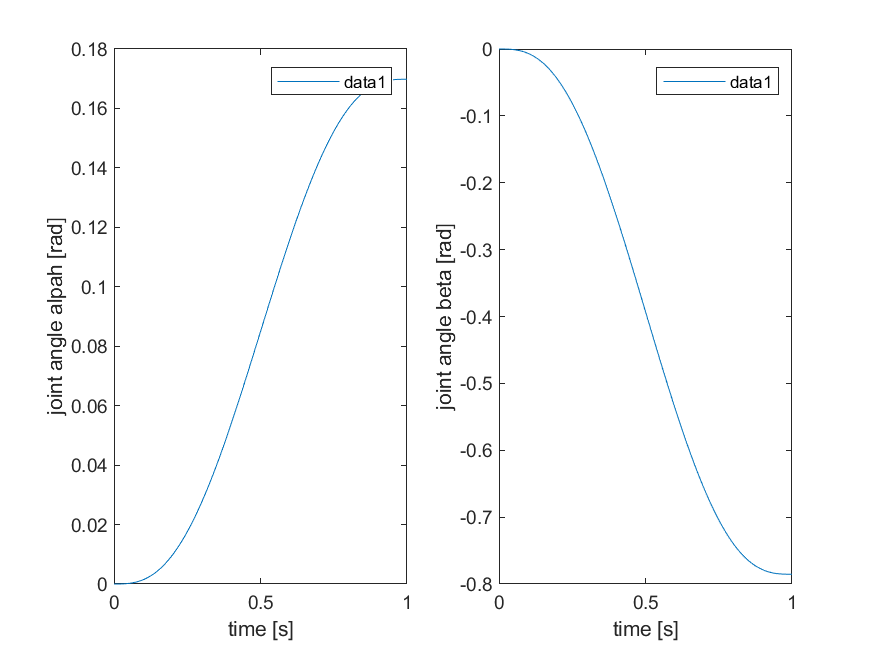
\includegraphics[width=0.95\textwidth]{Trajektorie.png}
	\caption{Trajektorie für \(\alpha\) und \(\beta\) }
\end{figure}

